\documentclass{article}
\usepackage[margin=1in]{geometry}
\usepackage{amsmath,amsthm,amssymb}
\usepackage{bbm,enumerate,mathtools}
\usepackage{tikz,pgfplots}
\usepackage{chessboard}
\usepackage[hidelinks]{hyperref}
\usepackage{multicol} % Problem 35
\usepackage{xstring} % Difficulty command
\usetikzlibrary{shapes.geometric}

\newenvironment{question}{\begin{trivlist}\item[\textbf{Question.}]}{\end{trivlist}}
\newenvironment{note}{\begin{trivlist}\item[\textbf{Note.}]}{\end{trivlist}}
\newenvironment{references}{\begin{trivlist}\item[\textbf{References.}]}{\end{trivlist}}
\newenvironment{related}{\begin{trivlist}\item[\textbf{Related.}]\end{trivlist}\begin{enumerate}}{\end{enumerate}}

\newcommand\score[1]{
\pgfmathsetmacro\pgfxa{#1+1}
\tikzstyle{scorestars}=[
  star,
  star points=5,
  star point ratio=2.25,
  draw,
  inner sep=3pt,
  anchor=outer point 5
]
  \begin{tikzpicture}[baseline]
    \draw[opacity=0] (0,-0.5) rectangle (0,0.2); % Workaround for whitespace at the bottom.
    \foreach \i in {1,...,4} {
      \pgfmathparse{(\i<=#1?"yellow":"gray")}
      \edef\starcolor{\pgfmathresult}
      \draw (\i*4.5ex,0) node[name=star\i,scorestars,fill=\starcolor]  {};
    }
  \end{tikzpicture}
}

\newcommand{\difficulty}[1]{%
  \IfEqCase{#1}{%
      {1}{
        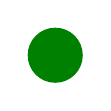
\begin{tikzpicture}[scale=0.7, baseline=0.9mm]%
          \definecolor{slopegreen}{rgb}{0.0, 0.5, 0.0}%
          \fill[slopegreen] (0.5,0.5) circle (0.5);%
        \end{tikzpicture}%
      }%
      {2}{
        
\begin{tikzpicture}[scale=0.7, baseline=0.9mm]%
          \definecolor{slopeblue}{rgb}{0.0, 0.44, 1.00}
          \fill[slopeblue] (0,0) rectangle (1,1);%
        \end{tikzpicture}%
      }%
      {3}{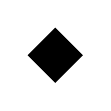
\begin{tikzpicture}[scale=0.7, baseline=0.9mm]\fill (0,0.5)--(0.5, 0)--(1,0.5)--(0.5,1)--cycle; \end{tikzpicture}}%
      {4}{
\begin{tikzpicture}[scale=0.7, baseline=0.9mm]\fill (0.25,0)--(0,0.5)--(0.25,1)--(0.5,0.5)--cycle; \fill (0.75,0)--(0.5,0.5)--(0.75,1)--(1,0.5)--cycle;\end{tikzpicture}}%
      % you can add more cases here as desired
  }[\PackageError{difficulty}{Undefined difficulty level: #1}{}]%
}%
\newcommand{\rating}[2]{\difficulty{#1}\\\score{#2}\\}


\begin{document}

\rating{3}{4}
The chromatic polynomial of a graph $G$, $\chi_G(n)$ gives the number of ways
to color the vertices of the graph such that no two vertices of the same color
are connected by an edge.

\begin{figure}[ht!]
  \centering
  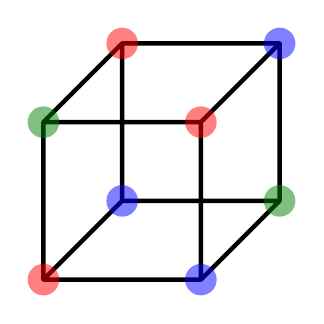
\begin{tikzpicture}
    \draw[ultra thick, line join=round]
      (1,3)--(3,3)--(2,2)--(0,2)--cycle
      (1,1)--(3,1)--(2,0)--(0,0)--cycle
      (0,0)--(0,2)
      (1,1)--(1,3)
      (2,0)--(2,2)
      (3,1)--(3,3);
    \fill[opacity=0.5, red]
      (0,0) circle (0.2)
      (2,2) circle (0.2)
      (1,3) circle (0.2);
    \fill[opacity=0.5, blue]
      (2,0) circle (0.2)
      (1,1) circle (0.2)
      (3,3) circle (0.2);
    \fill[opacity=0.5, green!50!black]
      (0,2) circle (0.2)
      (3,1) circle (0.2);
  \end{tikzpicture}
  ~
  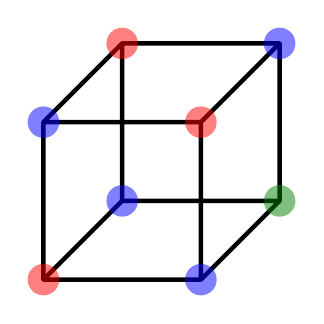
\begin{tikzpicture}
    \draw[ultra thick, line join=round]
      (1,3)--(3,3)--(2,2)--(0,2)--cycle
      (1,1)--(3,1)--(2,0)--(0,0)--cycle
      (0,0)--(0,2)
      (1,1)--(1,3)
      (2,0)--(2,2)
      (3,1)--(3,3);
    \fill[opacity = 0.5, red]
      (0,0) circle (0.2)
      (2,2) circle (0.2)
      (1,3) circle (0.2);
    \fill[opacity = 0.5, blue]
      (0,2) circle (0.2)
      (1,1) circle (0.2)
      (2,0) circle (0.2)
      (3,3) circle (0.2);
    \fill[opacity = 0.5, green!50!black]
      (3,1) circle (0.2);

  \end{tikzpicture}
  ~
  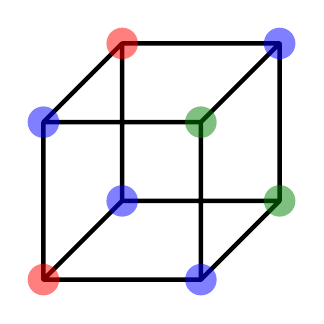
\begin{tikzpicture}
    \draw[ultra thick, line join=round]
      (1,3)--(3,3)--(2,2)--(0,2)--cycle
      (1,1)--(3,1)--(2,0)--(0,0)--cycle
      (0,0)--(0,2)
      (1,1)--(1,3)
      (2,0)--(2,2)
      (3,1)--(3,3);
    \fill[opacity=0.5, red]
      (0,0) circle (0.2)
      (1,3) circle (0.2);
    \fill[opacity=0.5, blue]
      (0,2) circle (0.2)
      (1,1) circle (0.2)
      (2,0) circle (0.2)
      (3,3) circle (0.2);
    \fill[opacity=0.5, green!50!black]
      (2,2) circle (0.2)
      (3,1) circle (0.2);
  \end{tikzpicture}
  \caption{Three examples of $3$-colorings of the cube. The chromatic polynomial
  of the cubic graph is ${\chi_{Q_3}(n) =
  a(n) = n^8 - 12n^7 + 66n^6 - 214n^5 + 441n^4 - 572n^3 + 423n^2 - 133n}$.}
\end{figure}

\begin{question}
  Is there a way to generate the chromatic polynomial of an $n$-cube in
  polynomial time with respect to $n$?
\end{question}

\begin{related}
  \item What about up to permutations of the colors and/or isometries of the cube?
  \item What about simplices, cross-polytopes, and demicubes?
  \item What about other polytopes such as associahedra, permutahedra, and
    the 24-, 120-, and 600-cells?
\end{related}

\begin{references}
  \item \url{https://math.stackexchange.com/q/3632156/121988}
  \item \url{https://oeis.org/A334230}
\end{references}
\end{document}
